\documentclass{article}
\usepackage{fancyhdr}
\usepackage{ctex}
\usepackage{listings}
\usepackage{graphicx}
\usepackage[a4paper, body={18cm,22cm}]{geometry}
\usepackage{amsmath,amssymb,amstext,wasysym,enumerate,graphicx}
\usepackage{float,abstract,booktabs,indentfirst,amsmath}
\usepackage{array}
\usepackage{booktabs}
\usepackage{multirow}
\usepackage{url}
\usepackage{diagbox}
\usepackage{hyperref}
\usepackage{listings}
\renewcommand\arraystretch{1.4}
\usepackage{indentfirst}
\setlength{\parindent}{2em}
\usepackage{enumitem}
\usepackage{accsupp}
\setmonofont{Consolas}
\usepackage{listings}
\usepackage{xcolor}
\usepackage{makecell}
\setCJKmonofont{黑体}
\newcommand\emptyaccsupp[1]{\BeginAccSupp{ActualText={}}#1\EndAccSupp{}}
\lstset{
    % language = C,
    xleftmargin = 3em,xrightmargin = 3em, aboveskip = 1em,
	backgroundcolor = \color{white}, % 背景色
	basicstyle = \small\ttfamily, % 基本样式 + 小号字体
	rulesepcolor= \color{gray}, % 代码块边框颜色
	breaklines = true, % 代码过长则换行
	numbers = left, % 行号在左侧显示
	numberstyle=\emptyaccsupp,
    numbersep = 14pt, 
    keywordstyle=\color{purple}\bfseries, % 关键字颜色
    commentstyle =\color{red!50!green!50!blue!60}, % 注释颜色
    stringstyle = \color{red}, % 字符串颜色
    morekeywords={ASSERT, int64_t, uint32_t},
	% frame = shadowbox, % 用(带影子效果)方框框住代码块
	frame = single, % 用(带影子效果)方框框住代码块
	showspaces = false, % 不显示空格
	columns = fixed, % 字间距固定
  framesep=1em
} 
\lstset{
    sensitive=true,
    moreemph={ASSERT, NULL}, emphstyle=\color{red}\bfseries,
    moreemph=[2]{int64_t, uint32_t, tid_t, uint8_t, int16_t, uint16_t, int32_t, size_t}, emphstyle=[2]\color{purple}\bfseries,
    }
%--------------------页眉--------------------%
\pagestyle{fancy}
\fancyhead[L]{}
\fancyhead[R]{}
\fancyhead[C]{《数据库系统及应用实践》课程实验报告}
\fancyfoot[C]{-\thepage-}
\renewcommand{\headrulewidth}{1.5pt}
%--------------------标题--------------------%
\begin{document}
\begin{center}
  \LARGE{{\textbf{\heiti 《数据库系统及应用实践》课程实验报告}}}

  \vspace{0.5em}

  \large 实验1:在 \texttt{Docker} 环境下使用 \texttt{MySQL}
  \begin{table}[H]
    \centering
    \begin{tabular}{p{2cm}p{2cm}<{\centering}p{0.4cm}p{2cm}p{3cm}<{\centering}p{0.4cm}p{2cm}p{3cm}<{\centering}}
      姓\qquad 名: & 李鹏达 & \quad & 学\qquad 号: & 10225101460 & \quad & 完成日期: & 2024年3月7日 \\ \cline{2-2} \cline{5-5} \cline{8-8}
    \end{tabular}
  \end{table}
\end{center}
% \rule{\textwidth}{1pt}
%--------------------正文--------------------%
\section{实验目标}
\begin{enumerate}[noitemsep]
  \item 学习 {\tt{Docker}} 环境的原理和基本操作
  \item 能够通过 {\tt{Docker}} 容器启动 {\tt{MySQL}} 数据库实例
  \item 掌握连接和操作{\tt{MySQL}} 数据库的基本命令
\end{enumerate}

\section{实验过程记录}

\subsection{安装 \texttt{Docker}}

我的实验环境是 \texttt{Ubuntu 22.04 LTS on Windows 10 x86\_64},在这里,我选择按照官网文档(\url{https://docs.docker.com/engine/install/ubuntu/})安装 \texttt{Docker}。

首先,添加 \texttt{Docker} 的 \texttt{apt} 源:

\begin{lstlisting}[language=bash]
# Add Docker's official GPG key:
sudo apt-get update
sudo apt-get install ca-certificates curl
sudo install -m 0755 -d /etc/apt/keyrings
sudo curl -fsSL https://download.docker.com/linux/ubuntu/gpg -o /etc/apt/keyrings/docker.asc
sudo chmod a+r /etc/apt/keyrings/docker.asc

# Add the repository to Apt sources:
echo \
  "deb [arch=$(dpkg --print-architecture) signed-by=/etc/apt/keyrings/docker.asc] https://download.docker.com/linux/ubuntu \
  $(. /etc/os-release && echo "$VERSION_CODENAME") stable" | \
  sudo tee /etc/apt/sources.list.d/docker.list > /dev/null
sudo apt-get update
\end{lstlisting}

然后使用 \texttt{apt} 安装 \texttt{Docker}:

\begin{lstlisting}[language=bash]
sudo apt-get install docker-ce docker-ce-cli containerd.io docker-buildx-plugin docker-compose-plugin
\end{lstlisting}

待安装完成后,运行命令以检查 \texttt{Docker}是否安装成功:

\begin{lstlisting}[language=bash]
sudo docker run hello-world
\end{lstlisting}

输出结果如下图所示,说明 \texttt{Docker} 安装成功。

\begin{figure}[H]
  \centering
  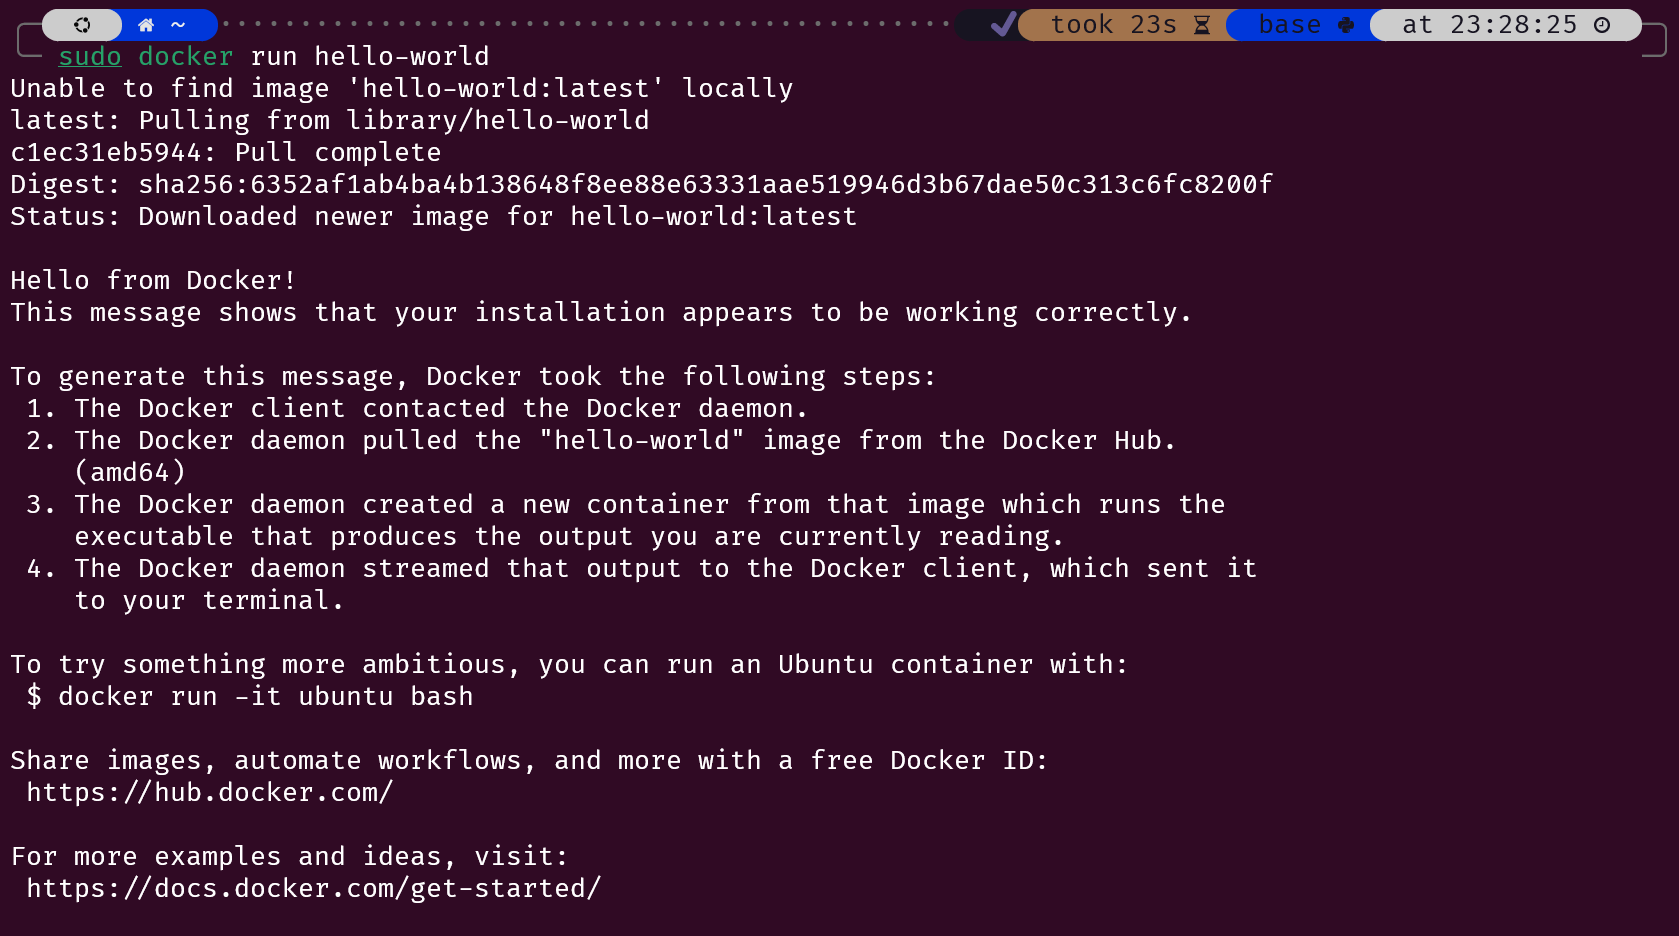
\includegraphics[width=0.9\textwidth]{img/1.png}
  \caption{检查 \texttt{Docker} 是否安装成功}
\end{figure}

\subsection{在容器中启动 \texttt{MySQL} 示例}

首先,创建一个 \texttt{dbcourse} 文件夹,并在其中创建一个 \texttt{datadir} 文件夹:

\begin{lstlisting}[language=bash]
mkdir dbcourse
cd dbcourse
mkdir datadir
\end{lstlisting}

然后拉取 \texttt{MySQL}镜像:

\begin{lstlisting}[language=bash]
sudo docker pull mysql:8.2.0
\end{lstlisting}

结果如下图所示:

\begin{figure}[H]
  \centering
  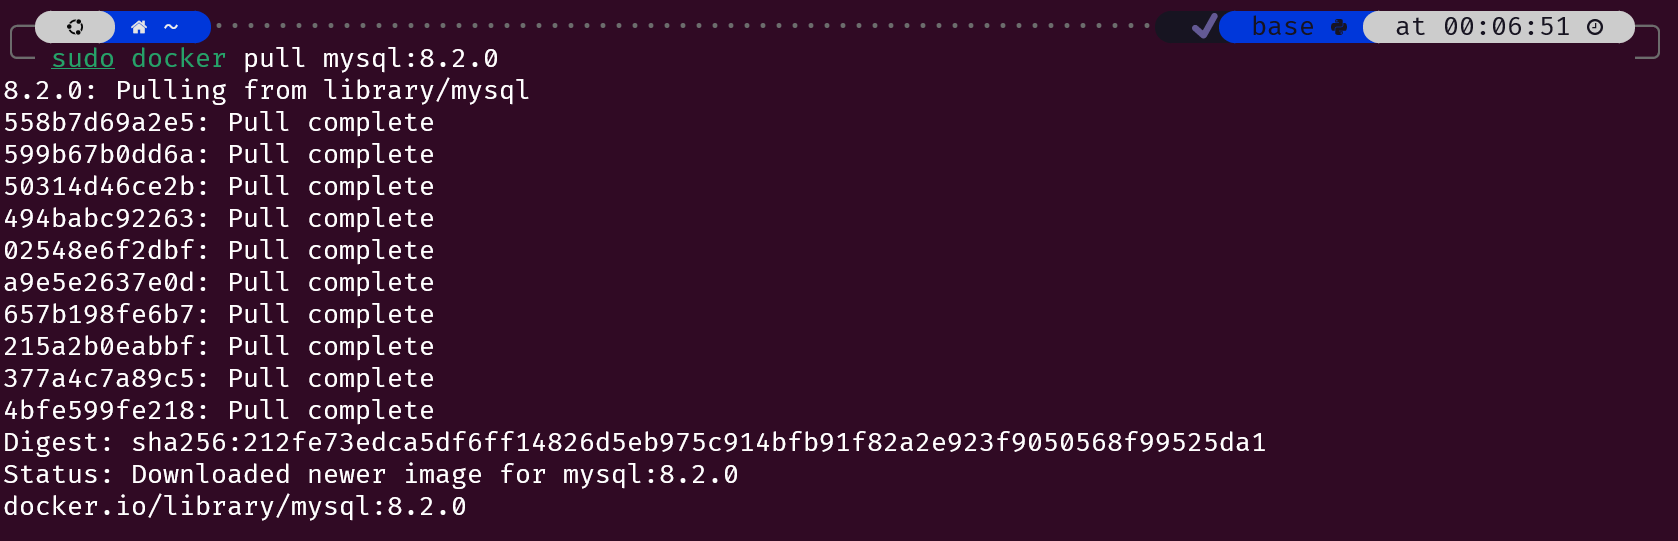
\includegraphics[width=0.9\textwidth]{img/2.png}
  \caption{拉取 \texttt{MySQL} 镜像}
\end{figure}

接下来,使用如下命令启动一个 \texttt{MySQL} 容器:

\begin{lstlisting}[language=bash]
sudo docker run --name dbcourse -v ./datadir:/var/lib/mysql -e MYSQL_ROOT_PASSWORD=password -d -p 53306:3306 mysql:8.2.0
\end{lstlisting}

这个命令将会创建一个名为 \texttt{dbcourse} 的容器,并将容器内的 \texttt{/var/lib/mysql} 文件夹映射到宿主机的 \texttt{./datadir} 文件夹,设置 \texttt{root} 用户的密码为 \texttt{password},将容器的 \texttt{3306} 端口映射到宿主机的 \texttt{53306} 端口。

结果如下图所示:

\begin{figure}[H]
  \centering
  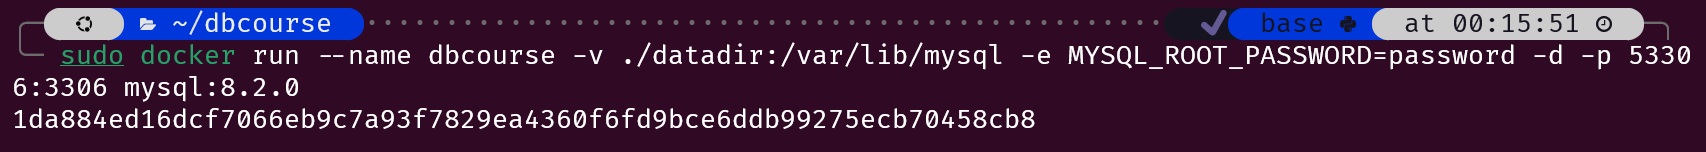
\includegraphics[width=0.9\textwidth]{img/3.png}
  \caption{创建容器}
\end{figure}

使用 \texttt{docker ps} 命令可以看到这个容器正在运行:

\begin{figure}[H]
  \centering
  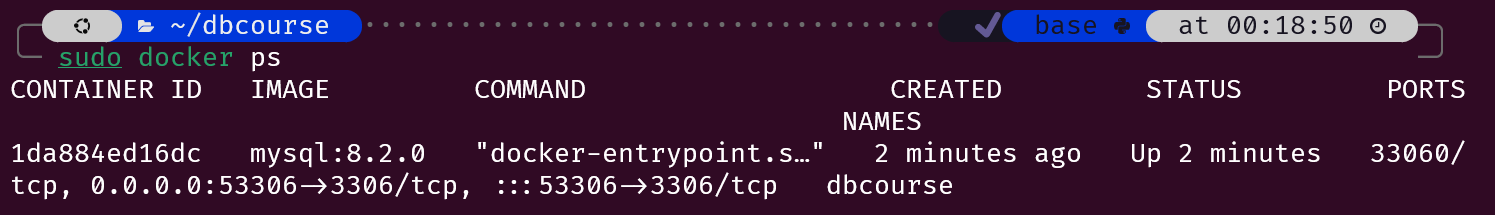
\includegraphics[width=0.9\textwidth]{img/4.png}
  \caption{查看运行中的容器}
\end{figure}

\subsection{对 \texttt{MySQL} 数据库进行操作}

执行如下命令,启动容器内的一个 \texttt{bash} 终端:

\begin{lstlisting}[language=bash]
sudo docker exec -it dbcourse bash
\end{lstlisting}

结果如下:

\begin{figure}[H]
  \centering
  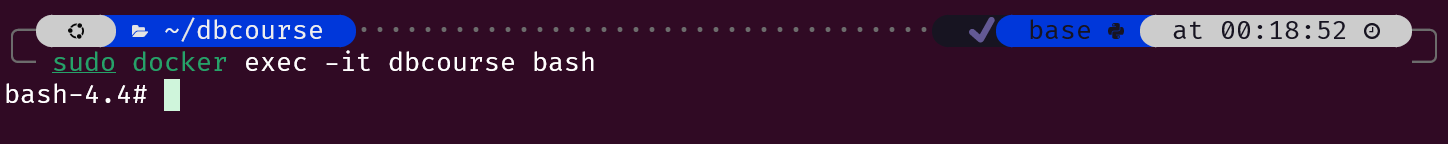
\includegraphics[width=0.9\textwidth]{img/5.png}
  \caption{启动容器内的 \texttt{bash} 终端}
\end{figure}

使用命令登录 \texttt{MySQL} 数据库:

\begin{lstlisting}[language=bash]
mysql --user=root --password=password
\end{lstlisting}

\begin{figure}[H]
  \centering
  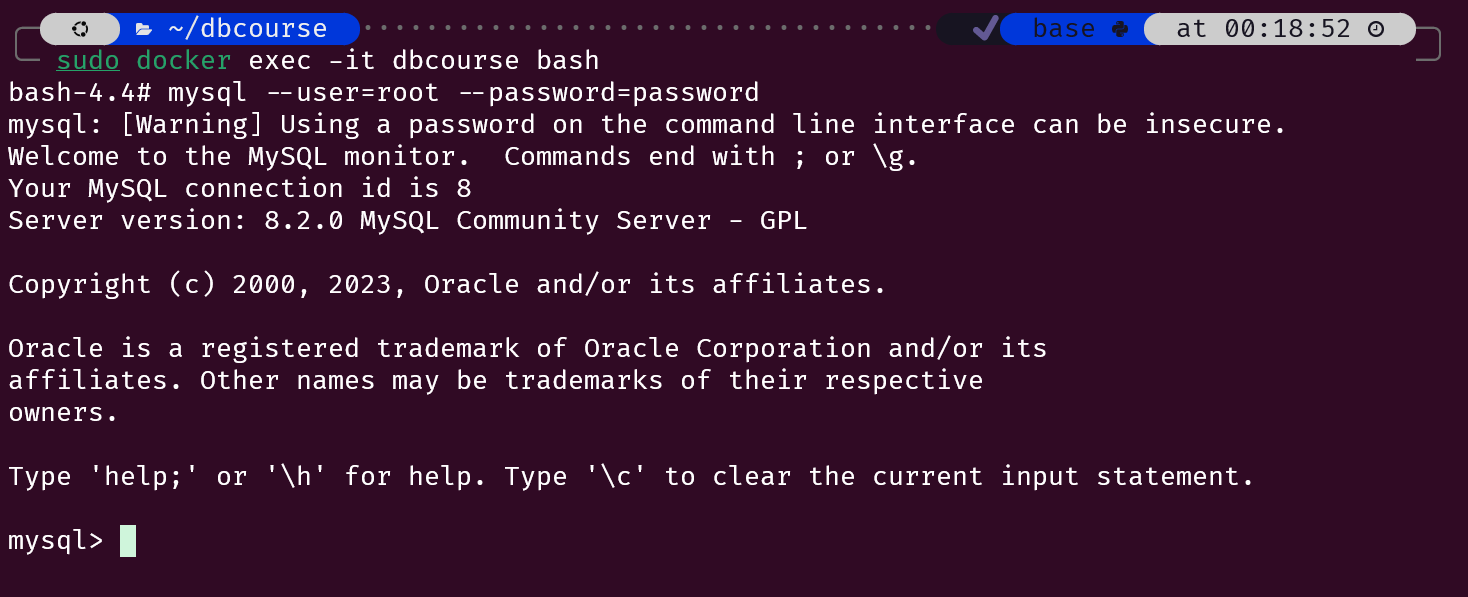
\includegraphics[width=0.9\textwidth]{img/6.png}
  \caption{登录 \texttt{MySQL}}
\end{figure}

执行 \texttt{help} 命令,可以看到 \texttt{MySQL} 的帮助信息:

\begin{lstlisting}[language=sql]
help;
\end{lstlisting}

\begin{figure}[H]
  \centering
  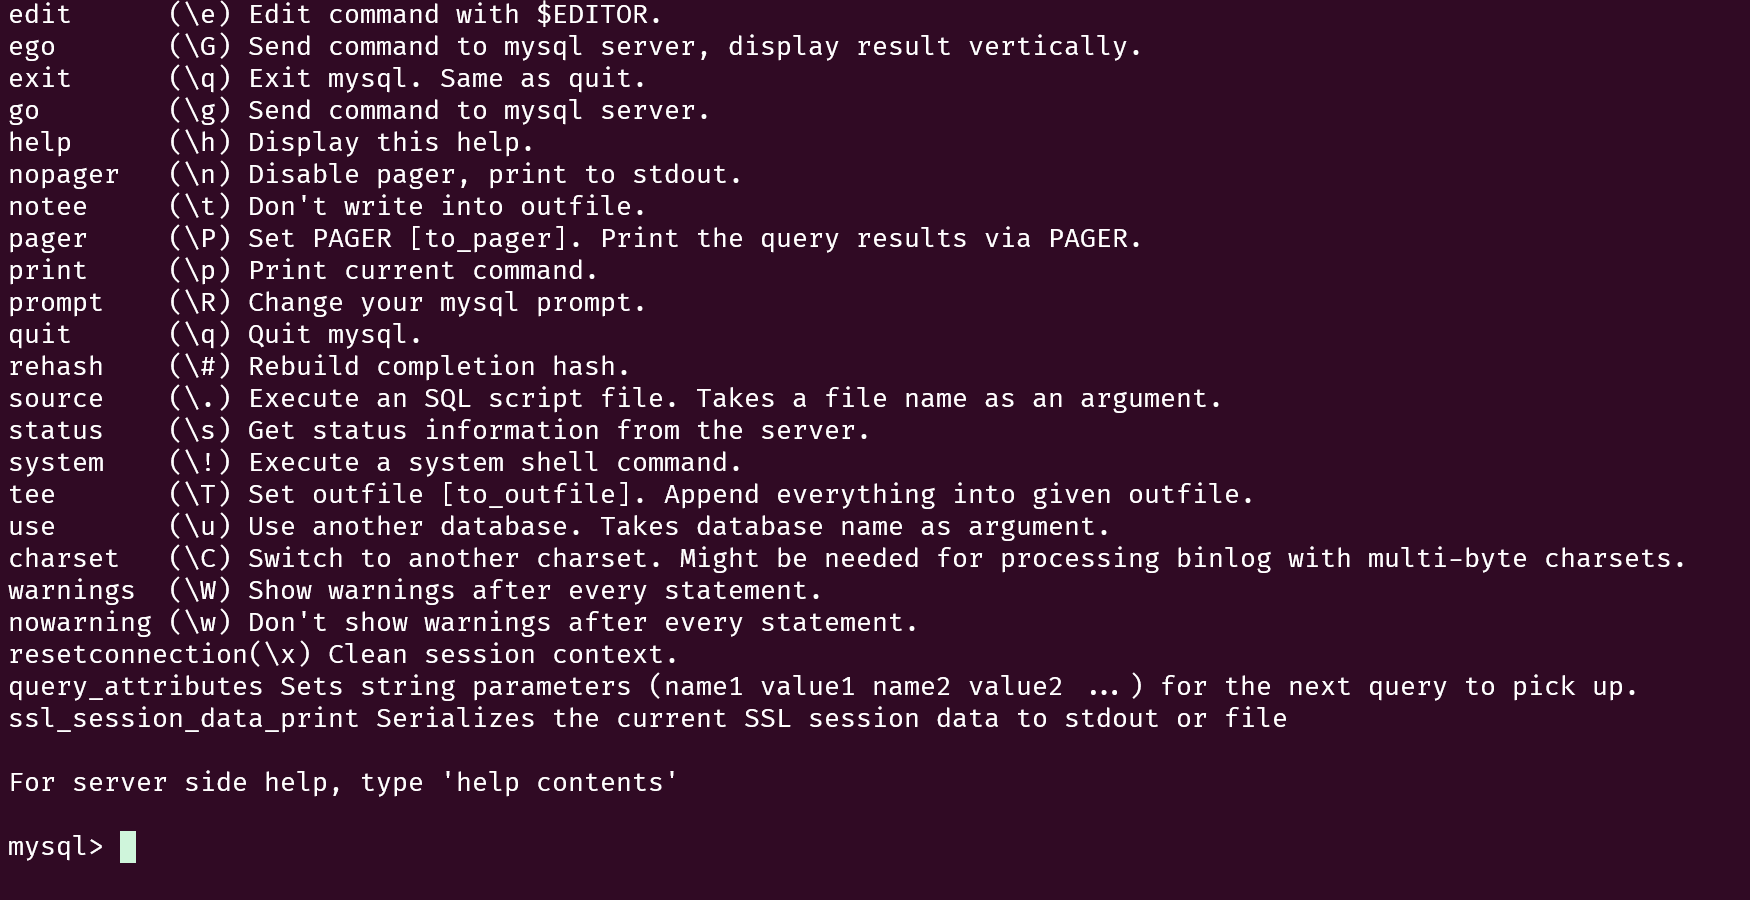
\includegraphics[width=0.9\textwidth]{img/7.png}
  \caption{\texttt{help} 命令}
\end{figure}

创建一个名为 \texttt{dbcourse}的数据库对象

\begin{lstlisting}[language=sql]
create database dbcourse;
\end{lstlisting}

\begin{figure}[H]
  \centering
  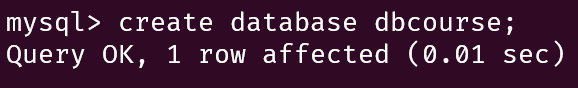
\includegraphics[width=12cm]{img/8.png}
  \caption{创建数据库对象}
\end{figure}

查看系统中所有的数据库对象

\begin{lstlisting}[language=sql]
show databases;
\end{lstlisting}

\begin{figure}[H]
  \centering
  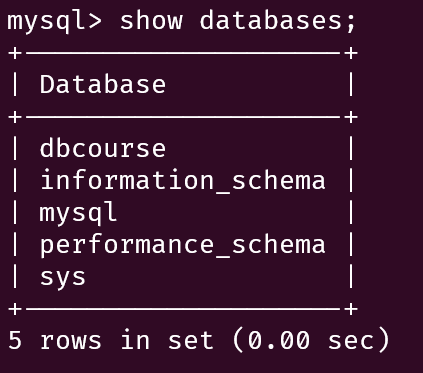
\includegraphics[width=8cm]{img/9.png}
  \caption{查看所有的数据库对象}
\end{figure}

将当前使用的数据库设置为 \texttt{dbcourse}

\begin{lstlisting}[language=sql]
use dbcourse;
\end{lstlisting}

\begin{figure}[H]
  \centering
  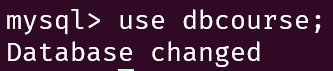
\includegraphics[width=0.3\textwidth]{img/10.png}
  \caption{设置当前使用的数据库}
\end{figure}

接下来,执行下列 \texttt{SQL}语句,在\texttt{dbcourse} 数据库中创建数据表

\begin{lstlisting}[language=sql]
create table classroom(
    building varchar(15),
    room_number varchar(7),
    capacity numeric(4,0),
    primary key (building, room_number)
);
create table department(
    dept_name varchar(20),
    building varchar(15),
    budget numeric(12,2) check (budget > 0),
    primary key (dept_name)
);
create table course(
    course_id varchar(8),
    title varchar(50),
    dept_name varchar(20),
    credits numeric(2,0) check (credits > 0),
    primary key (course_id),
    foreign key (dept_name) references department (dept_name)
    on delete set null
);
create table instructor(
    ID varchar(5),
    name varchar(20) not null,
    dept_name varchar(20),
    salary numeric(8,2) check (salary > 29000),
    primary key (ID),
    foreign key (dept_name) references department (dept_name)
    on delete set null
);
create table section(
    course_id varchar(8),
    sec_id varchar(8),
    semester varchar(6) check (semester in
    ('Fall', 'Winter', 'Spring', 'Summer')),
    year numeric(4,0) check (year > 1701 and year < 2100),
    building varchar(15),
    room_number varchar(7),
    time_slot_id varchar(4),
    primary key (course_id, sec_id, semester, year),
    foreign key (course_id) references course (course_id) on delete cascade,
    foreign key (building, room_number)
    references classroom (building, room_number) on delete set null
);
create table teaches(
    ID varchar(5),
    course_id varchar(8),
    sec_id varchar(8),
    semester varchar(6),
    year numeric(4,0),
    primary key (ID, course_id, sec_id, semester, year),
    foreign key (course_id, sec_id, semester, year)
    references section (course_id, sec_id, semester, year)
    on delete cascade,
    foreign key (ID) references instructor (ID) on delete cascade
);
create table student(
    ID varchar(5),
    name varchar(20) not null,
    dept_name varchar(20),
    tot_cred numeric(3,0) check (tot_cred >= 0),
    primary key (ID),
    foreign key (dept_name) references department (dept_name)
    on delete set null
);
create table takes(
    ID varchar(5),
    course_id varchar(8),
    sec_id varchar(8),
    semester varchar(6),
    year numeric(4,0),
    grade varchar(2),
    primary key (ID, course_id, sec_id, semester, year),
    foreign key (course_id, sec_id, semester, year)
    references section (course_id, sec_id, semester, year)
    on delete cascade,
    foreign key (ID) references student (ID) on delete cascade
);
create table advisor(
    s_ID varchar(5),
    i_ID varchar(5),
    primary key (s_ID),
    foreign key (i_ID) references instructor (ID) on delete set null,
    foreign key (s_ID) references student (ID) on delete cascade
);
create table time_slot(
    time_slot_id varchar(4),
    day varchar(1),
    start_hr numeric(2) check (start_hr >= 0 and start_hr < 24),
    start_min numeric(2) check (start_min >= 0 and start_min < 60),
    end_hr numeric(2) check (end_hr >= 0 and end_hr < 24),
    end_min numeric(2) check (end_min >= 0 and end_min < 60),
    primary key (time_slot_id, day, start_hr, start_min)
);
create table prereq(
    course_id varchar(8),
    prereq_id varchar(8),
    primary key (course_id, prereq_id),
    foreign key (course_id) references course (course_id) on delete cascade,
    foreign key (prereq_id) references course (course_id)
);
\end{lstlisting}

然后查看 \texttt{dbcourse} 数据库中所有的数据表

\begin{lstlisting}[language=sql]
show tables;
\end{lstlisting}

\begin{figure}[H]
  \centering
  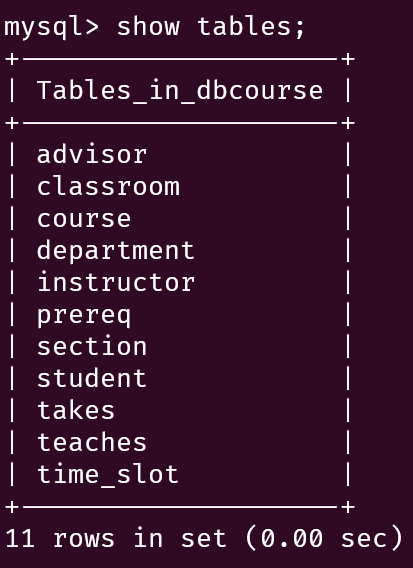
\includegraphics[width=0.3\textwidth]{img/11.png}
  \caption{查看所有的表}
\end{figure}

接下来,执行下列 \texttt{SQL}语句,向数据表中插入数据:

\begin{lstlisting}[language=sql]
insert into classroom values ('Packard', '101', '500');
insert into classroom values ('Painter', '514', '10');
insert into classroom values ('Taylor', '3128', '70');
insert into classroom values ('Watson', '100', '30');
insert into classroom values ('Watson', '120', '50');
insert into department values ('Biology', 'Watson', '90000');
insert into department values ('Comp. Sci.', 'Taylor', '100000');
insert into department values ('Elec. Eng.', 'Taylor', '85000');
insert into department values ('Finance', 'Painter', '120000');
insert into department values ('History', 'Painter', '50000');
insert into department values ('Music', 'Packard', '80000');
insert into department values ('Physics', 'Watson', '70000');
insert into course values ('BIO-101', 'Intro. to Biology', 'Biology', '4');
insert into course values ('BIO-301', 'Genetics', 'Biology', '4');
insert into course values ('BIO-399', 'Computational Biology', 'Biology', '3');
insert into course values ('CS-101', 'Intro. to Computer Science', 'Comp. Sci.', '4');
insert into course values ('CS-190', 'Game Design', 'Comp. Sci.', '4');
insert into course values ('CS-315', 'Robotics', 'Comp. Sci.', '3');
insert into course values ('CS-319', 'Image Processing', 'Comp. Sci.', '3');
insert into course values ('CS-347', 'Database System Concepts', 'Comp. Sci.', '3');
insert into course values ('EE-181', 'Intro. to Digital Systems', 'Elec. Eng.', '3');
insert into course values ('FIN-201', 'Investment Banking', 'Finance', '3');
insert into course values ('HIS-351', 'World History', 'History', '3');
insert into course values ('MU-199', 'Music Video Production', 'Music', '3');
insert into course values ('PHY-101', 'Physical Principles', 'Physics', '4');
insert into instructor values ('10101', 'Srinivasan', 'Comp. Sci.', '65000');
insert into instructor values ('12121', 'Wu', 'Finance', '90000');
insert into instructor values ('15151', 'Mozart', 'Music', '40000');
insert into instructor values ('22222', 'Einstein', 'Physics', '95000');
insert into instructor values ('32343', 'El Said', 'History', '60000');
insert into instructor values ('33456', 'Gold', 'Physics', '87000');
insert into instructor values ('45565', 'Katz', 'Comp. Sci.', '75000');
insert into instructor values ('58583', 'Califieri', 'History', '62000');
insert into instructor values ('76543', 'Singh', 'Finance', '80000');
insert into instructor values ('76766', 'Crick', 'Biology', '72000');
insert into instructor values ('83821', 'Brandt', 'Comp. Sci.', '92000');
insert into instructor values ('98345', 'Kim', 'Elec. Eng.', '80000');
insert into section values ('BIO-101', '1', 'Summer', '2017', 'Painter', '514', 'B');
insert into section values ('BIO-301', '1', 'Summer', '2018', 'Painter', '514', 'A');
insert into section values ('CS-101', '1', 'Fall', '2017', 'Packard', '101', 'H');
insert into section values ('CS-101', '1', 'Spring', '2018', 'Packard', '101', 'F');
insert into section values ('CS-190', '1', 'Spring', '2017', 'Taylor', '3128', 'E');
insert into section values ('CS-190', '2', 'Spring', '2017', 'Taylor', '3128', 'A');
insert into section values ('CS-315', '1', 'Spring', '2018', 'Watson', '120', 'D');
insert into section values ('CS-319', '1', 'Spring', '2018', 'Watson', '100', 'B');
insert into section values ('CS-319', '2', 'Spring', '2018', 'Taylor', '3128', 'C');
insert into section values ('CS-347', '1', 'Fall', '2017', 'Taylor', '3128', 'A');
insert into section values ('EE-181', '1', 'Spring', '2017', 'Taylor', '3128', 'C');
insert into section values ('FIN-201', '1', 'Spring', '2018', 'Packard', '101', 'B');
insert into section values ('HIS-351', '1', 'Spring', '2018', 'Painter', '514', 'C');
insert into section values ('MU-199', '1', 'Spring', '2018', 'Packard', '101', 'D');
insert into section values ('PHY-101', '1', 'Fall', '2017', 'Watson', '100', 'A');
insert into teaches values ('10101', 'CS-101', '1', 'Fall', '2017');
insert into teaches values ('10101', 'CS-315', '1', 'Spring', '2018');
insert into teaches values ('10101', 'CS-347', '1', 'Fall', '2017');
insert into teaches values ('12121', 'FIN-201', '1', 'Spring', '2018');
insert into teaches values ('15151', 'MU-199', '1', 'Spring', '2018');
insert into teaches values ('22222', 'PHY-101', '1', 'Fall', '2017');
insert into teaches values ('32343', 'HIS-351', '1', 'Spring', '2018');
insert into teaches values ('45565', 'CS-101', '1', 'Spring', '2018');
insert into teaches values ('45565', 'CS-319', '1', 'Spring', '2018');
insert into teaches values ('76766', 'BIO-101', '1', 'Summer', '2017');
insert into teaches values ('76766', 'BIO-301', '1', 'Summer', '2018');
insert into teaches values ('83821', 'CS-190', '1', 'Spring', '2017');
insert into teaches values ('83821', 'CS-190', '2', 'Spring', '2017');
insert into teaches values ('83821', 'CS-319', '2', 'Spring', '2018');
insert into teaches values ('98345', 'EE-181', '1', 'Spring', '2017');
insert into student values ('00128', 'Zhang', 'Comp. Sci.', '102');
insert into student values ('12345', 'Shankar', 'Comp. Sci.', '32');
insert into student values ('19991', 'Brandt', 'History', '80');
insert into student values ('23121', 'Chavez', 'Finance', '110');
insert into student values ('44553', 'Peltier', 'Physics', '56');
insert into student values ('45678', 'Levy', 'Physics', '46');
insert into student values ('54321', 'Williams', 'Comp. Sci.', '54');
insert into student values ('55739', 'Sanchez', 'Music', '38');
insert into student values ('70557', 'Snow', 'Physics', '0');
insert into student values ('76543', 'Brown', 'Comp. Sci.', '58');
insert into student values ('76653', 'Aoi', 'Elec. Eng.', '60');
insert into student values ('98765', 'Bourikas', 'Elec. Eng.', '98');
insert into student values ('98988', 'Tanaka', 'Biology', '120');
insert into takes values ('00128', 'CS-101', '1', 'Fall', '2017', 'A');
insert into takes values ('00128', 'CS-347', '1', 'Fall', '2017', 'A-');
insert into takes values ('12345', 'CS-101', '1', 'Fall', '2017', 'C');
insert into takes values ('12345', 'CS-190', '2', 'Spring', '2017', 'A');
insert into takes values ('12345', 'CS-315', '1', 'Spring', '2018', 'A');
insert into takes values ('12345', 'CS-347', '1', 'Fall', '2017', 'A');
insert into takes values ('19991', 'HIS-351', '1', 'Spring', '2018', 'B');
insert into takes values ('23121', 'FIN-201', '1', 'Spring', '2018', 'C+');
insert into takes values ('44553', 'PHY-101', '1', 'Fall', '2017', 'B-');
insert into takes values ('45678', 'CS-101', '1', 'Fall', '2017', 'F');
insert into takes values ('45678', 'CS-101', '1', 'Spring', '2018', 'B+');
insert into takes values ('45678', 'CS-319', '1', 'Spring', '2018', 'B');
insert into takes values ('54321', 'CS-101', '1', 'Fall', '2017', 'A-');
insert into takes values ('54321', 'CS-190', '2', 'Spring', '2017', 'B+');
insert into takes values ('55739', 'MU-199', '1', 'Spring', '2018', 'A-');
insert into takes values ('76543', 'CS-101', '1', 'Fall', '2017', 'A');
insert into takes values ('76543', 'CS-319', '2', 'Spring', '2018', 'A');
insert into takes values ('76653', 'EE-181', '1', 'Spring', '2017', 'C');
insert into takes values ('98765', 'CS-101', '1', 'Fall', '2017', 'C-');
insert into takes values ('98765', 'CS-315', '1', 'Spring', '2018', 'B');
insert into takes values ('98988', 'BIO-101', '1', 'Summer', '2017', 'A');
insert into takes values ('98988', 'BIO-301', '1', 'Summer', '2018', null);
insert into advisor values ('00128', '45565');
insert into advisor values ('12345', '10101');
insert into advisor values ('23121', '76543');
insert into advisor values ('44553', '22222');
insert into advisor values ('45678', '22222');
insert into advisor values ('76543', '45565');
insert into advisor values ('76653', '98345');
insert into advisor values ('98765', '98345');
insert into advisor values ('98988', '76766');
insert into time_slot values ('A', 'M', '8', '0', '8', '50');
insert into time_slot values ('A', 'W', '8', '0', '8', '50');
insert into time_slot values ('A', 'F', '8', '0', '8', '50');
insert into time_slot values ('B', 'M', '9', '0', '9', '50');
insert into time_slot values ('B', 'W', '9', '0', '9', '50');
insert into time_slot values ('B', 'F', '9', '0', '9', '50');
insert into time_slot values ('C', 'M', '11', '0', '11', '50');
insert into time_slot values ('C', 'W', '11', '0', '11', '50');
insert into time_slot values ('C', 'F', '11', '0', '11', '50');
insert into time_slot values ('D', 'M', '13', '0', '13', '50');
insert into time_slot values ('D', 'W', '13', '0', '13', '50');
insert into time_slot values ('D', 'F', '13', '0', '13', '50');
insert into time_slot values ('E', 'T', '10', '30', '11', '45 ');
insert into time_slot values ('E', 'R', '10', '30', '11', '45 ');
insert into time_slot values ('F', 'T', '14', '30', '15', '45 ');
insert into time_slot values ('F', 'R', '14', '30', '15', '45 ');
insert into time_slot values ('G', 'M', '16', '0', '16', '50');
insert into time_slot values ('G', 'W', '16', '0', '16', '50');
insert into time_slot values ('G', 'F', '16', '0', '16', '50');
insert into time_slot values ('H', 'W', '10', '0', '12', '30');
insert into prereq values ('BIO-301', 'BIO-101');
insert into prereq values ('BIO-399', 'BIO-101');
insert into prereq values ('CS-190', 'CS-101');
insert into prereq values ('CS-315', 'CS-101');
insert into prereq values ('CS-319', 'CS-101');
insert into prereq values ('CS-347', 'CS-101');
insert into prereq values ('EE-181', 'PHY-101');
\end{lstlisting}

执行下列\texttt{SQL}语句,查询每张数据表中的数据:

\begin{lstlisting}[language=sql]
select * from advisor;
select * from classroom;
select * from course;
select * from department;
select * from instructor;
select * from prereq;
select * from section;
select * from student;
select * from takes;
select * from teaches;
select * from time_slot;
\end{lstlisting}

\begin{figure}[H]
  \centering
  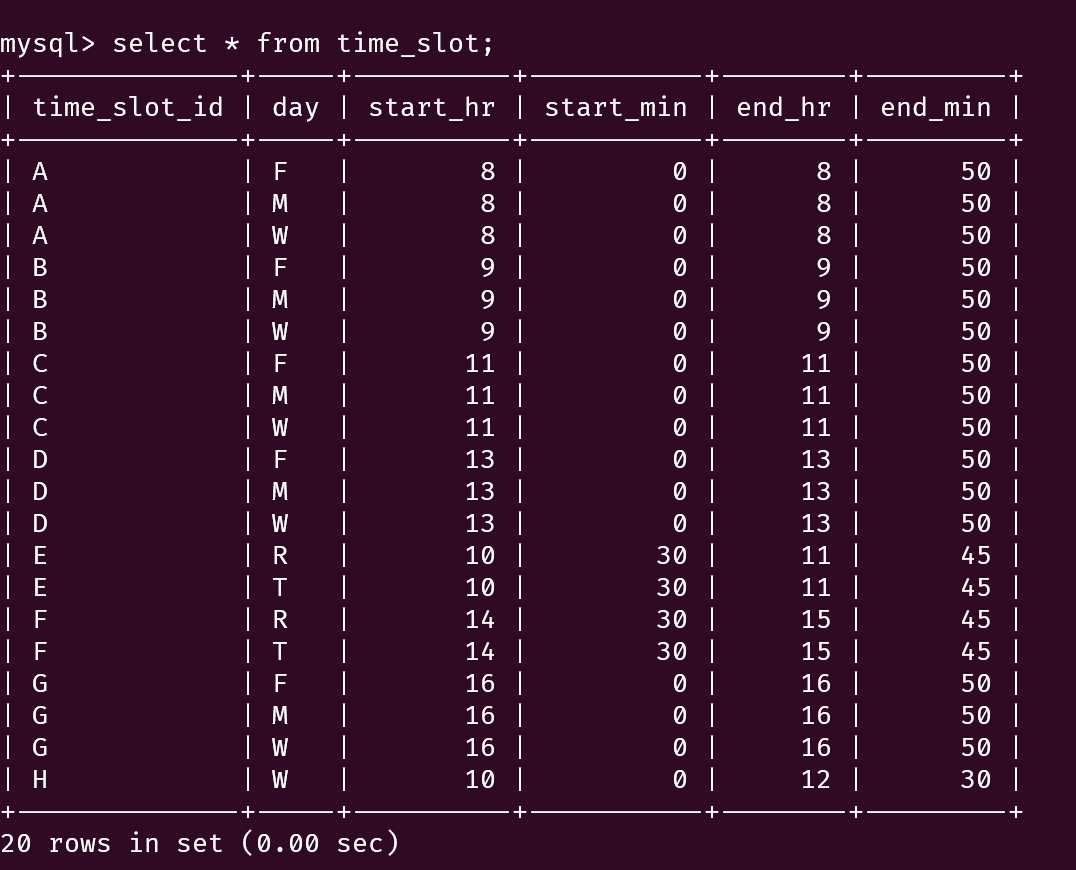
\includegraphics[width=0.6\textwidth]{img/12.png}
  \caption{查询表中的数据}
\end{figure}

使用 \texttt{describe} 命令查看数据表的结构:

\begin{lstlisting}[language=sql]
describe advisor;
\end{lstlisting}

\begin{figure}[H]
  \centering
  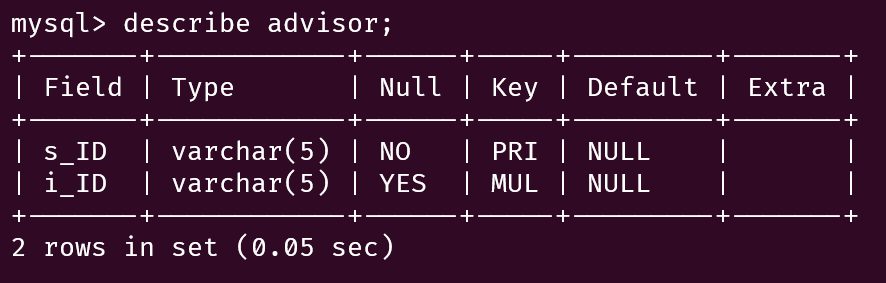
\includegraphics[width=0.6\textwidth]{img/13.png}
  \caption{查看表的结构}
\end{figure}

使用 \texttt{show index from} 语句查看数据表的索引信息

\begin{lstlisting}[language=sql]
show index from advisor;
\end{lstlisting}

\begin{figure}[H]
  \centering
  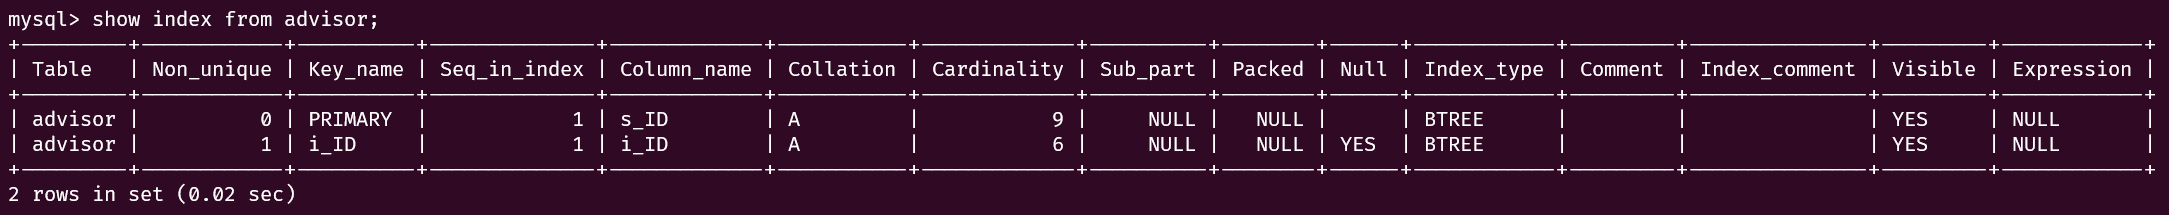
\includegraphics[width=\textwidth]{img/14.png}
  \caption{查看表的索引}
\end{figure}

将当前使用的数据库设置为 \texttt{mysql}

\begin{lstlisting}[language=sql]
use mysql;
\end{lstlisting}

查看 \texttt{mysql} 数据库中的所有数据表对象

\begin{lstlisting}[language=sql]
show tables;
\end{lstlisting}

\begin{figure}[H]
  \centering
  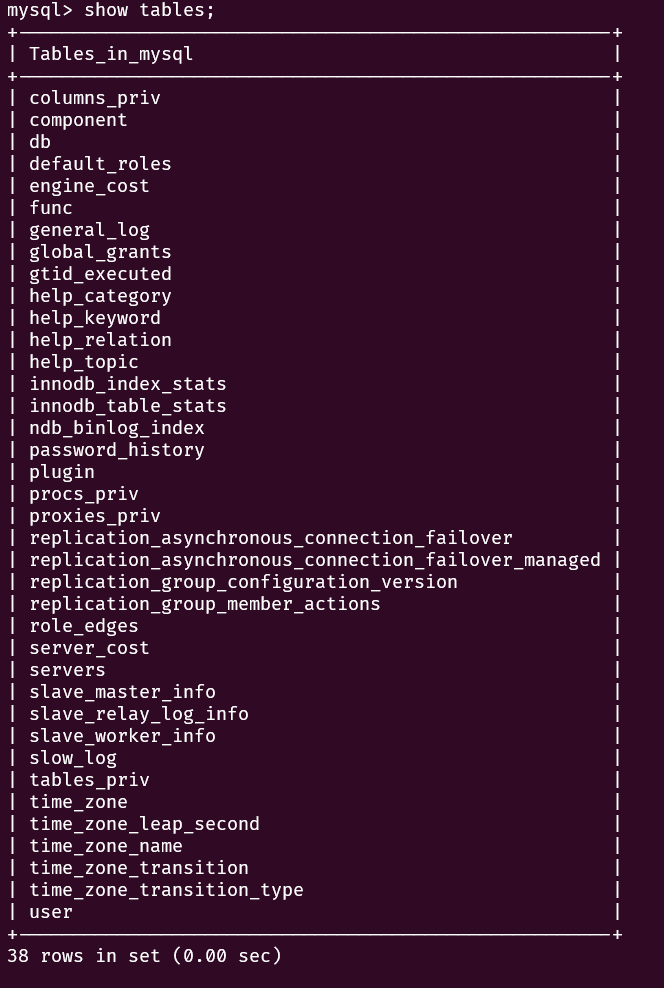
\includegraphics[width=0.4\textwidth]{img/15.png}
  \caption{查看 \texttt{mysql} 数据库中的所有数据表对象}
\end{figure}

查看数据库服务的状态

\begin{lstlisting}[language=sql]
show status;
\end{lstlisting}

\begin{figure}[H]
  \centering
  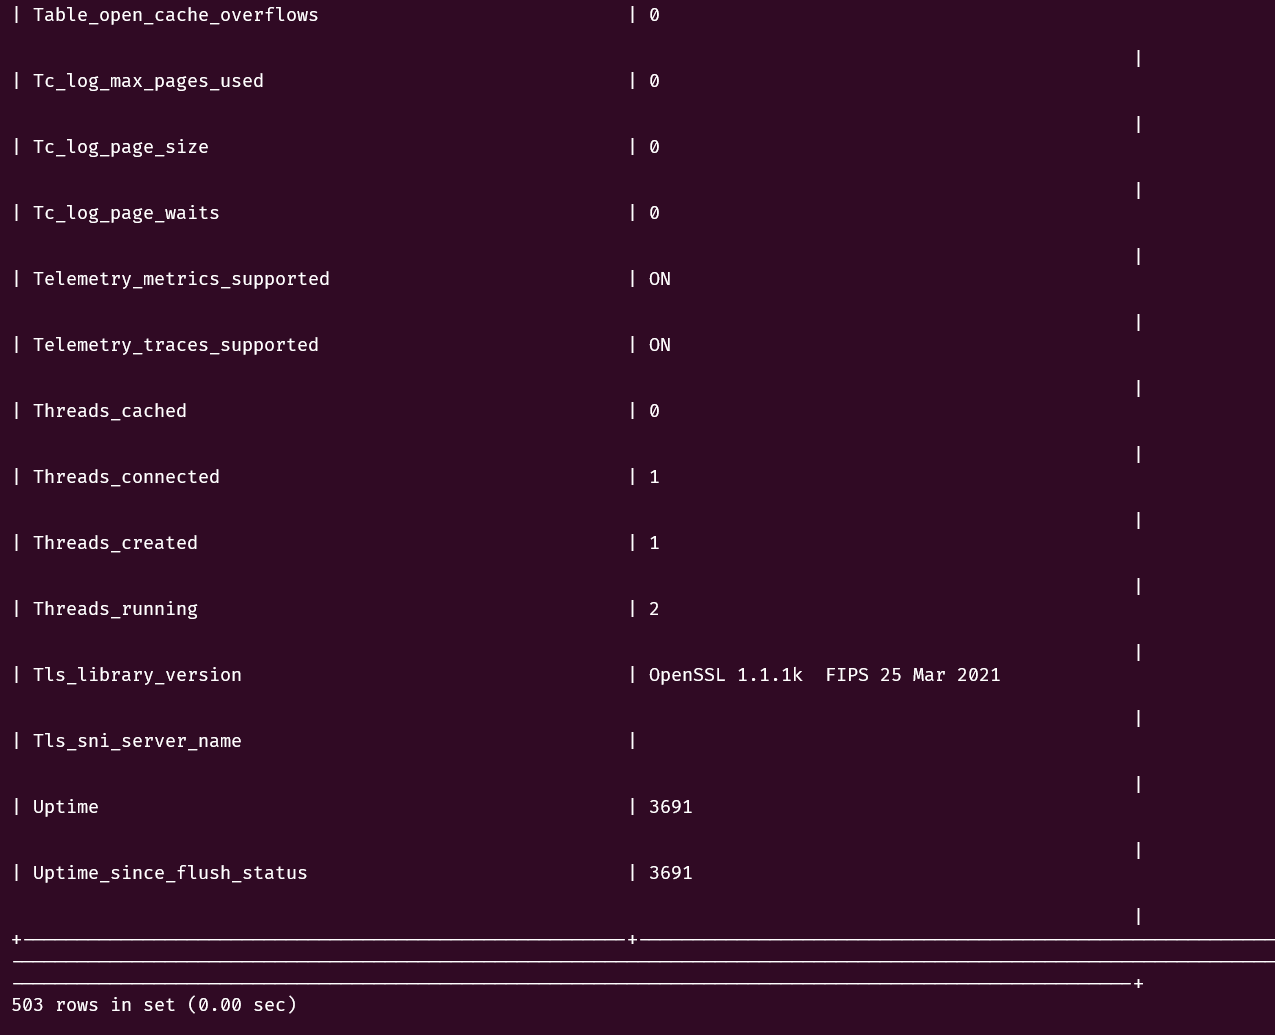
\includegraphics[width=0.9\textwidth]{img/16.png}
  \caption{查看数据库服务的状态}
\end{figure}

命令查询系统变量的值

\begin{lstlisting}[language=sql]
show variables;
\end{lstlisting}

\begin{figure}[H]
  \centering
  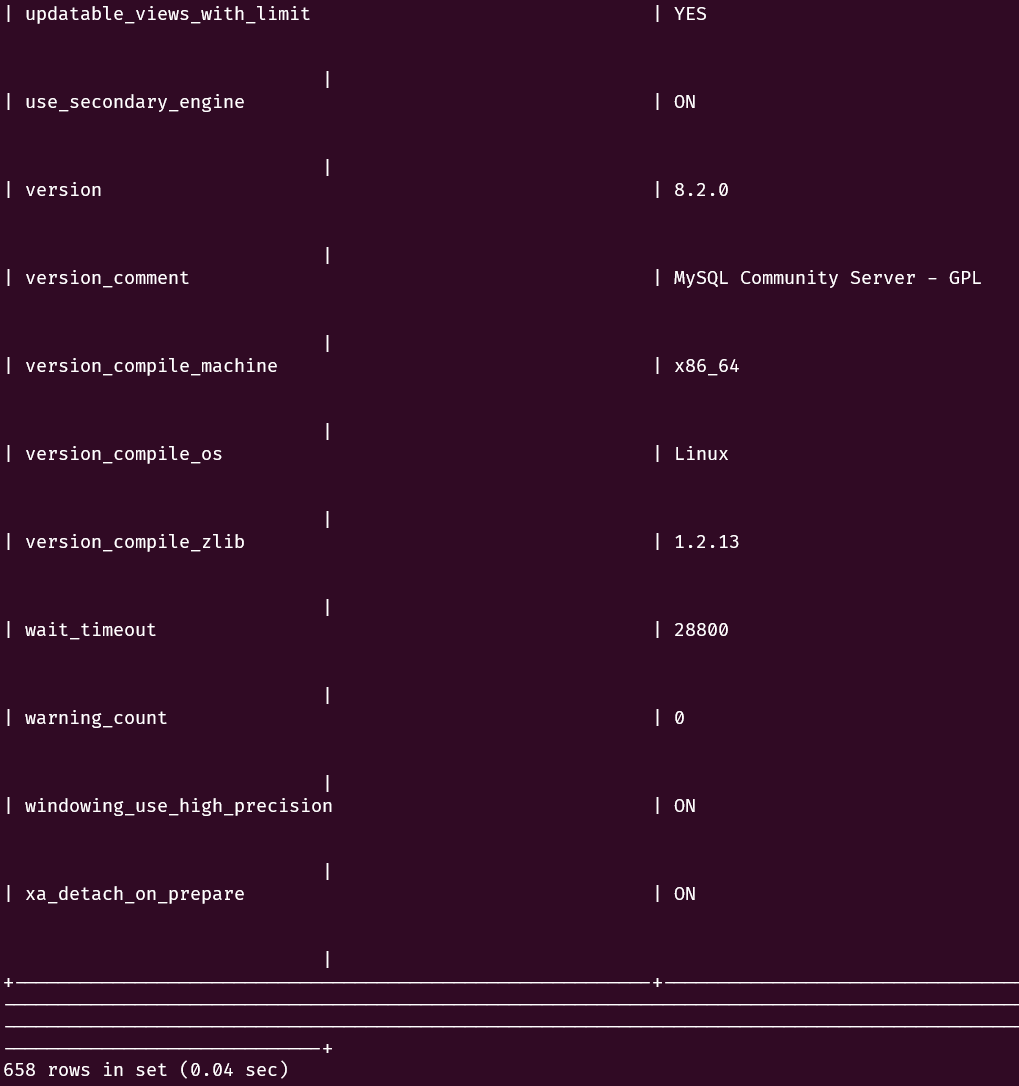
\includegraphics[width=0.7\textwidth]{img/17.png}
  \caption{查询系统变量的值}
\end{figure}

查询数据库服务的启动时间

\begin{lstlisting}[language=sql]
show global status like 'uptime';
\end{lstlisting}

\begin{figure}[H]
  \centering
  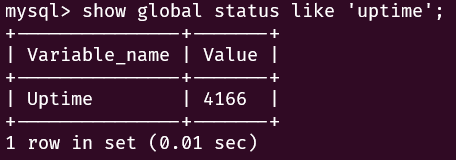
\includegraphics[width=0.55\textwidth]{img/18.png}
  \caption{查询数据库服务的启动时间}
\end{figure}

查询系统中的当前时间戳

\begin{lstlisting}[language=sql]
select unix_timestamp();
\end{lstlisting}

\begin{figure}[H]
  \centering
  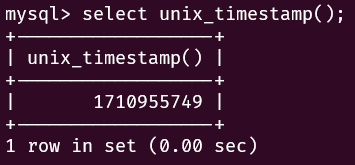
\includegraphics[width=0.5\textwidth]{img/19.png}
  \caption{查询系统中的当前时间戳}
\end{figure}

查询\texttt{MySQL}数据库服务的版本、当前日期、当前时间、当前用户和所使用的数据库

\begin{lstlisting}[language=sql]
select version(), curdate(), curtime(), current_user(), database();
\end{lstlisting}

\begin{figure}[H]
  \centering
  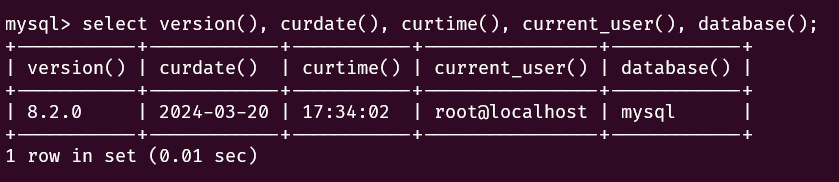
\includegraphics[width=0.9\textwidth]{img/20.png}
  \caption{查询相关内容}
\end{figure}

退出 \texttt{MySQL}

\begin{lstlisting}[language=sql]
exit;
\end{lstlisting}

退出 \texttt{bash}

\begin{lstlisting}[language=bash]
exit
\end{lstlisting}

\subsection{通过图形工具 \texttt{Navicat}连接并操作\texttt{MySQL}数据库}

在 \texttt{Navicat} 中新建一个连接,连接到 \texttt{MySQL} 数据库:

\begin{figure}[H]
\centering
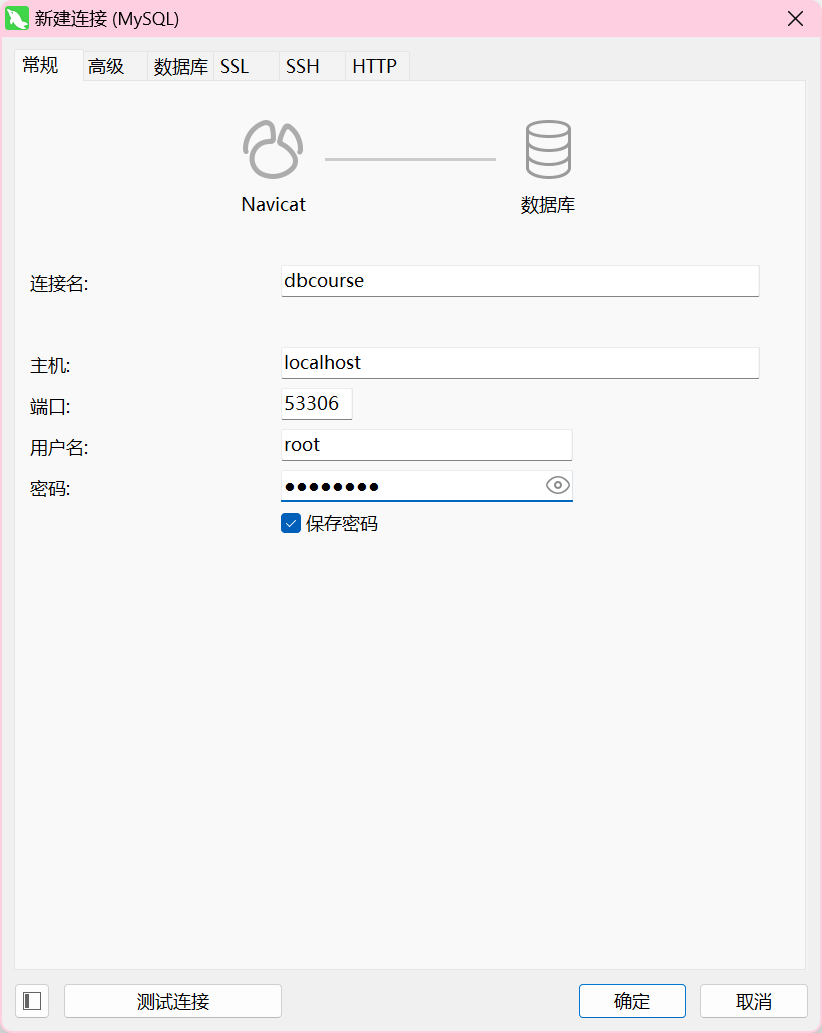
\includegraphics[width=0.5\textwidth]{img/21.png}
\caption{新建连接}
\end{figure}

连接成功后,通过 \texttt{Navicat}的图形界面查看数据表\texttt{instrctor}的结构和内容

\begin{figure}[H]
\centering
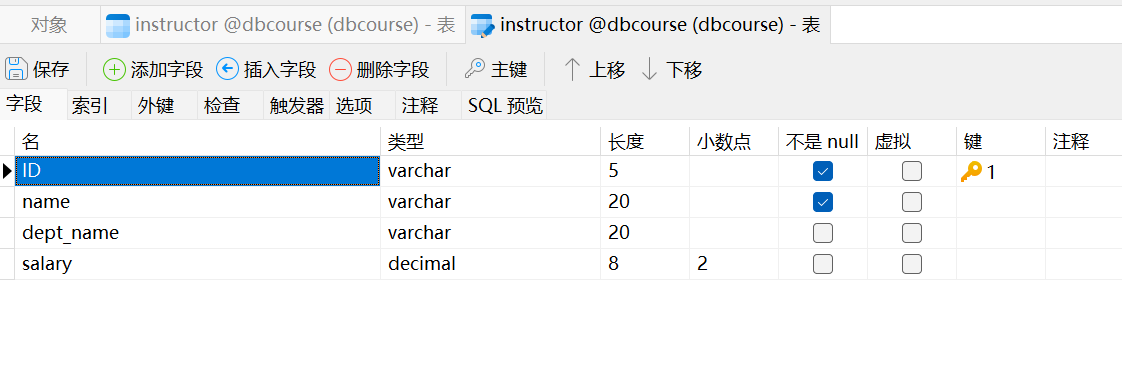
\includegraphics[width=0.9\textwidth]{img/22.png}
\caption{结构}
\end{figure}

\begin{figure}[H]
\centering
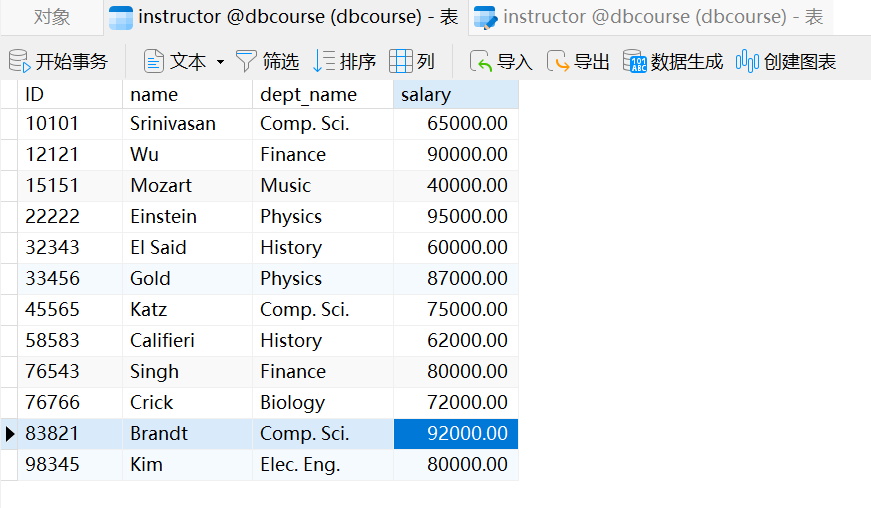
\includegraphics[width=0.9\textwidth]{img/23.png}
\caption{内容}
\end{figure}

通过\texttt{Navicat}的图形界面创建一个名为\texttt{dbtest}的数据库,在其中创建与\texttt{dbcourse}数据库相同的数据表,并导入相同的数据

\begin{figure}[H]
\centering
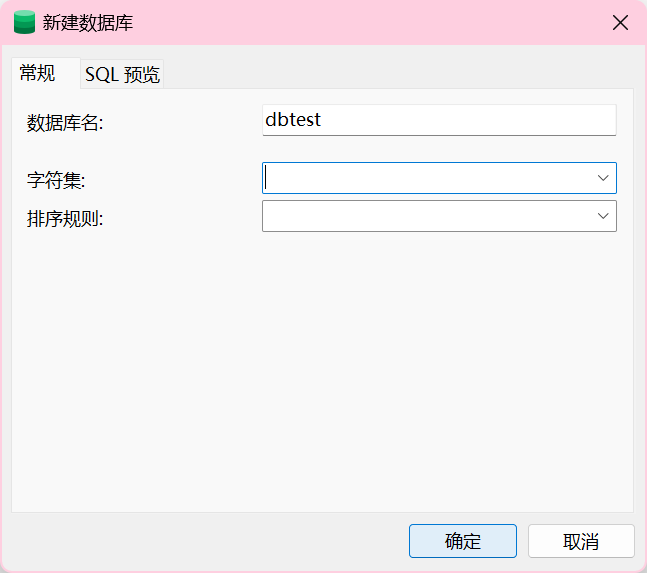
\includegraphics[width=0.4\textwidth]{img/24.png}
\caption{创建数据库}
\end{figure}

\begin{figure}[H]
\centering
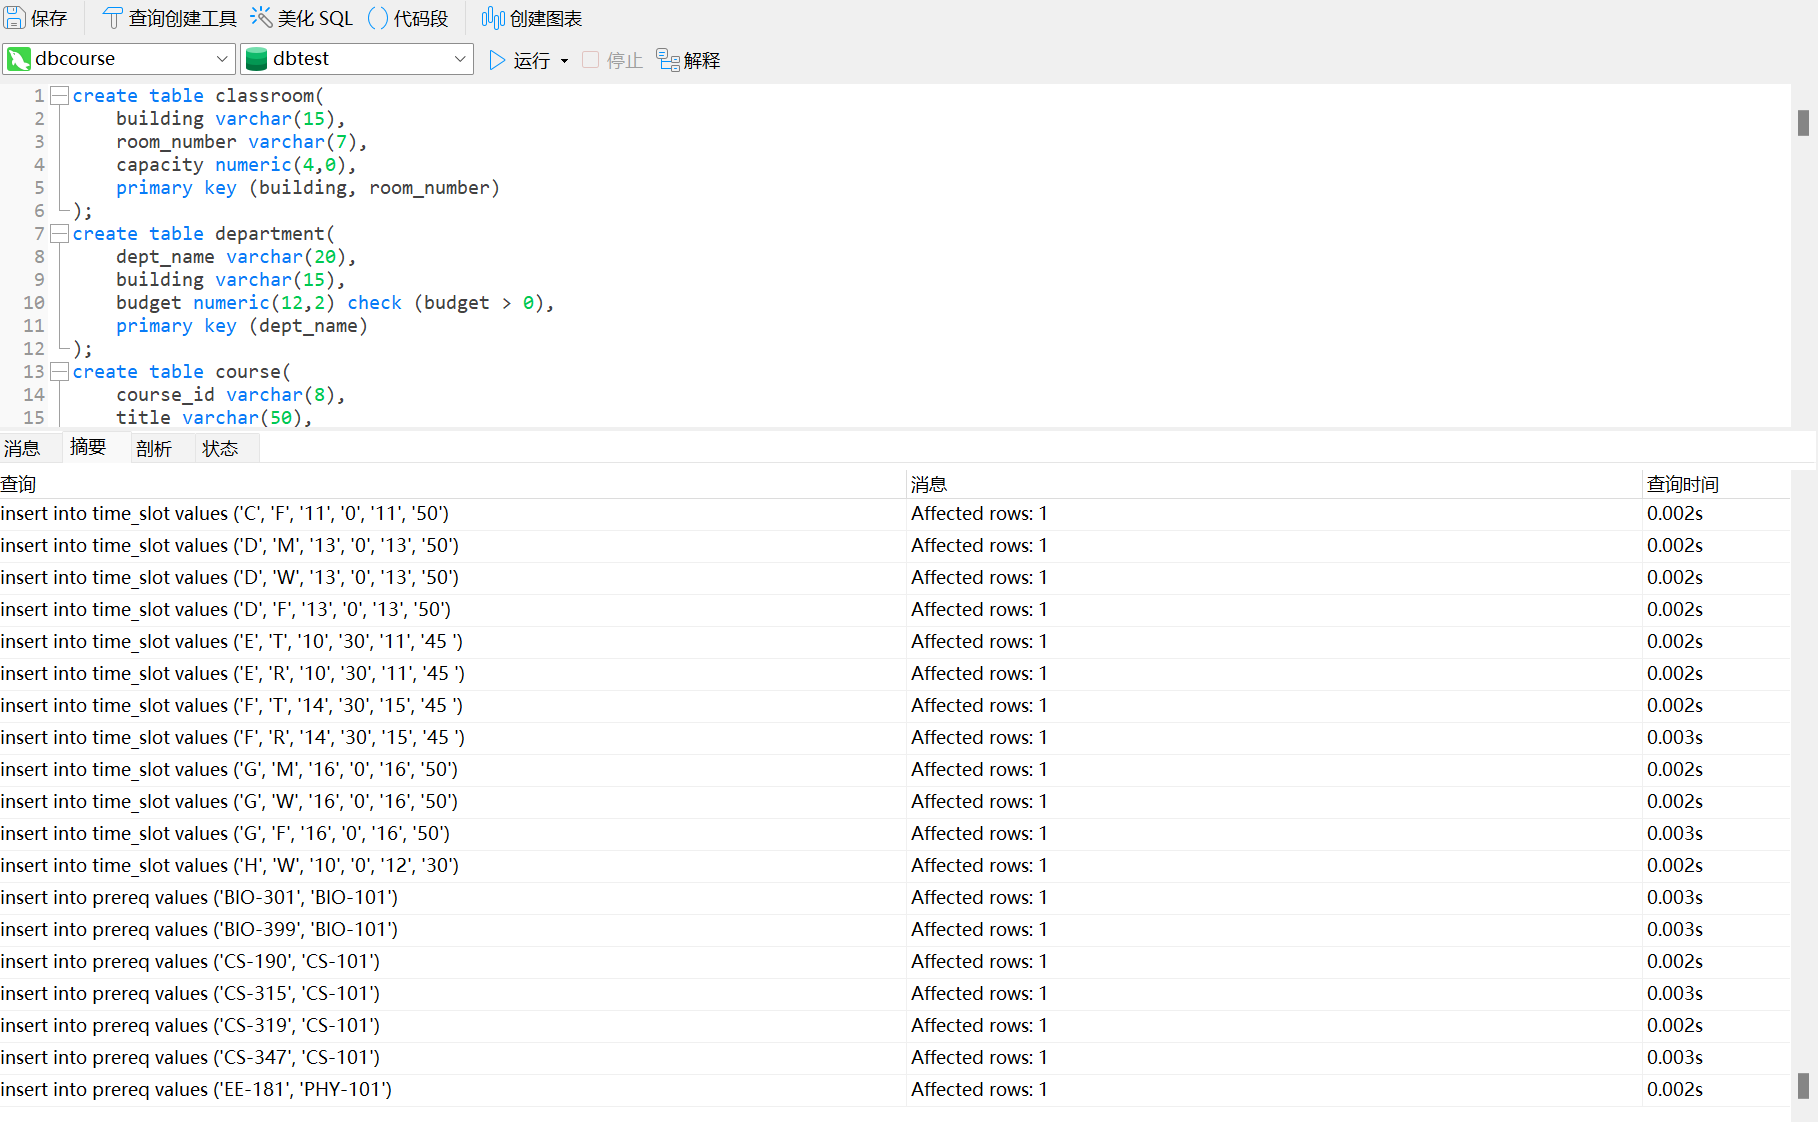
\includegraphics[width=0.9\textwidth]{img/25.png}
\caption{执行相关 \texttt{SQL} 语句}
\end{figure}

\subsection{\texttt{Docker}常用操作}

查看系统中所有的的容器信息

\begin{lstlisting}[language=bash]
sudo docker ps -a
\end{lstlisting}

\begin{figure}[H]
\centering
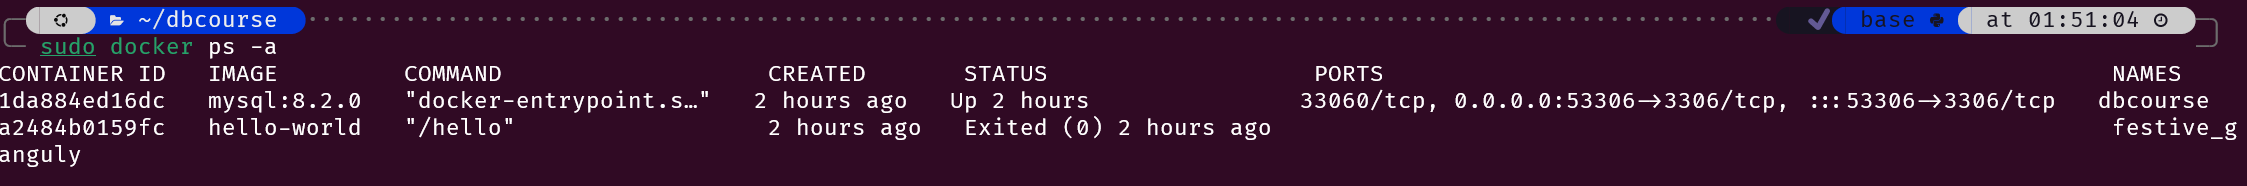
\includegraphics[width=0.9\textwidth]{img/26.png}
\caption{查看所有的的容器信息}
\end{figure}

将容器打包为镜像

\begin{lstlisting}[language=bash]
sudo docker commit dbcourse dbcourse:v1
\end{lstlisting}

\begin{figure}[H]
\centering
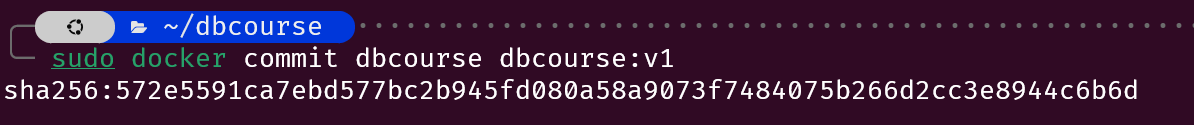
\includegraphics[width=0.9\textwidth]{img/27.png}
\caption{将容器打包为镜像}
\end{figure}

查看本地仓库中的镜像

\begin{lstlisting}[language=bash]
sudo docker images
\end{lstlisting}

\begin{figure}[H]
\centering
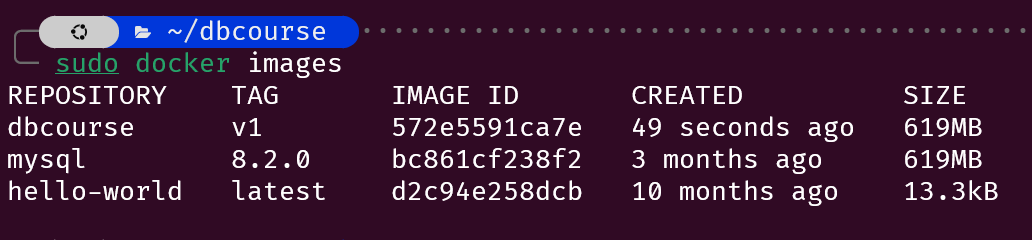
\includegraphics[width=0.7\textwidth]{img/28.png}
\caption{本地仓库中的镜像}
\end{figure}

将镜像\texttt{dbcourse}保存为文件

\begin{lstlisting}[language=bash]
sudo docker save -o dbcourse.tar dbcourse
\end{lstlisting}

\begin{figure}[H]
\centering
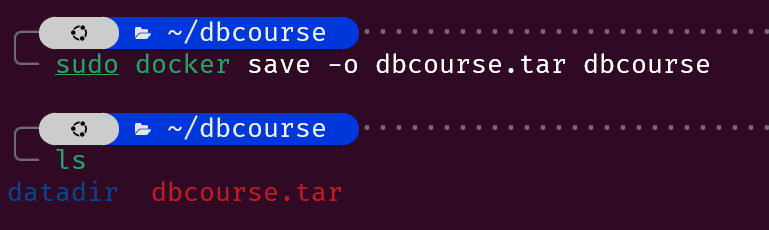
\includegraphics[width=0.5\textwidth]{img/29.png}
\caption{将镜像\texttt{dbcourse}保存为文件}
\end{figure}

将本地仓库中的镜像\texttt{dbcourse}删除

\begin{lstlisting}[language=bash]
sudo docker image rm dbcourse:v1
\end{lstlisting}

\begin{figure}[H]
\centering
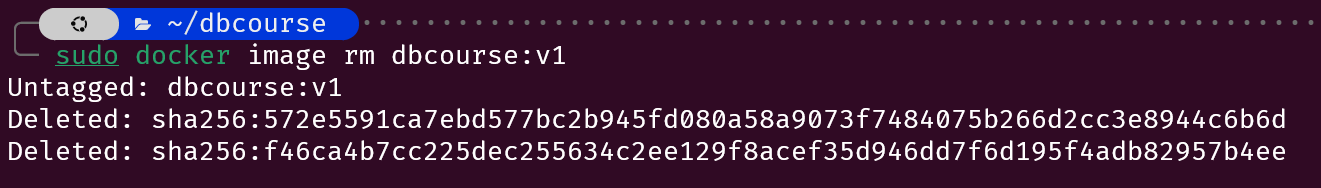
\includegraphics[width=0.6\textwidth]{img/30.png}
\caption{删除镜像}
\end{figure}

停止容器\texttt{dbcourse}的运行

\begin{lstlisting}[language=bash]
sudo docker stop dbcourse
\end{lstlisting}

\begin{figure}[H]
\centering

\includegraphics[width=0.6\textwidth]{img/31.png}
\caption{停止容器的运行}
\end{figure}

删除容器\texttt{dbcourse}

\begin{lstlisting}[language=bash]
sudo docker rm dbcourse
\end{lstlisting}

\begin{figure}[H]
\centering
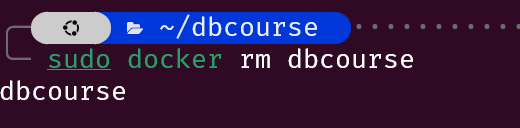
\includegraphics[width=0.6\textwidth]{img/32.png}
\caption{删除容器}
\end{figure}

将镜像文件加载到本地仓库

\begin{lstlisting}[language=bash]
sudo docker load --input dbcourse.tar
\end{lstlisting}

\begin{figure}[H]
\centering
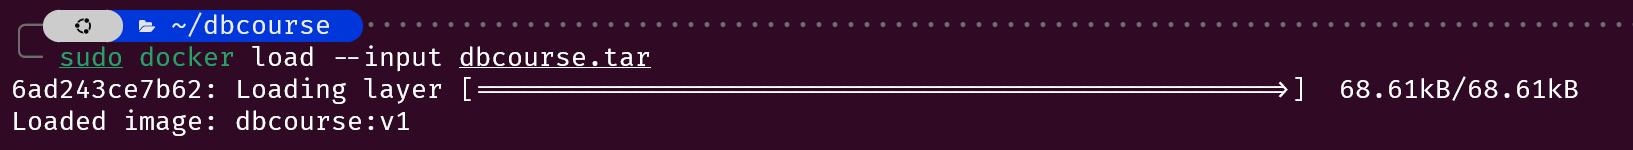
\includegraphics[width=0.9\textwidth]{img/33.png}
\caption{加载镜像文件}
\end{figure}

\section{存在的问题及解决方案}

在实验中,运行插入数据的\texttt{SQL}语句时,发生错误。经检查,是由于在复制\texttt{SQL}语句时,发生了在字符串中央的意外换行,导致\texttt{MySQL}无法识别。解决方案是将\texttt{SQL}语句复制到文本编辑器中,检查并删除意外的换行。

\section{实验小结}

通过本次实验,我学习了\texttt{Docker}的基本操作,掌握了通过\texttt{Docker}容器启动\texttt{MySQL}数据库实例,并连接和操作\texttt{MySQL}数据库的基本命令。同时,我还学会了使用\texttt{Navicat}连接并操作\texttt{MySQL}数据库,以及\texttt{Docker}的其他常用操作。这些知识对我今后的学习和工作都有很大的帮助。


\end{document}